In practice, the best performances for measuring impedance are obtained by using discrete Integrated Chips (IC) \cite{horowitz1989art}. For example, a waveform generator using the ICs AD5930 or AD5932 could be used to send a known sinusoidal signal to the SUT, which would then be measured by an ADC linked to a microcontroller that calculates the unknown impedance’s modulus and phase \cite{grossi2019electrical,Chowdhury2017}. A suitable Analog Front End (AFE) would be placed between the waveform from the generator and the SUT to better suit the specific application. \par

The specialized impedance analyzer IC AD5933 \cite{AD5933-documentation} can be used in a likewise fashion. This IC combines in a small package a sinusoidal voltage generator made from a 27-bits phase accumulator Direct Digital Synthesis (DDS) core and a Digital-to-Analog Converter (DAC), a TIA with a programmable gain, a 12-bits 1 MSPS ADC with a 100 kHz antialiasing filter, and an onboard Digital Signal Processing (DSP) unit which calculates a 1024 points Discrete Fourier Transform (DFT) with a Multiplier Accumulator (MAC) \cite{horowitz1989art}. Its functionalized diagram is illustrated in \autoref{fig:AD5933_diagram}. After the calculations, it yields the 16-bits real and imaginary impedance components through an I2C communication protocol \cite{horowitz1989art}, which can then be used to deduce the magnitude and phase of the SUT’s impedance:
\begin{equation}
   \lvert Z \rvert = \sqrt{Re(Z)+Im(Z)}
\end{equation}
\begin{equation}
   \theta = atan(\frac{Im(Z)}{Re(Z)})
\end{equation}
\begin{figure}[h]
    \centering
    \includegraphics[width=1\textwidth]{AD5933_diagram}
    \caption{Functional bloc-diagram of the AD5933 IC \cite{AD5933-documentation}.}
    \label{fig:AD5933_diagram}
\end{figure}
As explained by \citep{Chabowski2015}, the AD5933 IC suffers from multiple inherent defects, which can mostly be accounted for by a careful design of the AFE. Firstly, a serial resistance exists at the output transmit stage, which limits the lower bound of impedance measurement. The addition of a buffer between the transmit stage and the SUT helps to reduce to a minimum this parasitic serial resistance. \par

Secondly, the ADC suffers from a dead zone which can affect the measurement for voltages at the ADC’s input lower than 15 mV. Adding multiple switchable resistances for the TIA’s feedback resistance can solve this problem and makes it so that the tension at the ADC is pushed further to increasingly high and increasingly low values of SUT’s impedance, hopefully outside of the bounds of the given application \cite{Chabowski2015,horowitz1989art}. See \autoref{sec:PGA}. \par

Thirdly, the transmit stage provides varying Direct Current (DC) bias which must be accounted for to not saturate the op-amps. This can be done with a DC canceller circuit \cite{horowitz1989art}. In its simplest form, only a High-Pass filter (HPF) would suffice, but this configuration suffers from long measurement time at low frequency. HPFs are generally made with resistors and capacitors in a RC filter, which suffer from a long settling time caused by the transitory state of the HPFs. Considering that “the time constant of the RC filter has to be significantly longer than the longest period of the excitation voltage”\cite{Chabowski2015} in order to obtain a decent precision, the settling time can become unsatisfactorily high for low excitation frequency \cite{horowitz1989art}. \citep{Chabowski2015} proposed a novel DC canceller based on a positive and negative peak detector to reduce the measurement time. This circuit has been chosen by the author (K.Bouzid,2022) to be used in the final design of the EcoChip2 in \citep{das2020ecochip}, and will be described later in \autoref{app:Ecochip}. \par

Fourthly, the DFT introduces discontinuities in the digital calculations that affect the impedance measurement. The AD5933 implements a single-point DFT, which means that the analysis frequency running inside the MAC core should be at the same frequency of that of the output excitation signal. A smooth transition between the period of the excitation signal of the SUT and the DDS generator signal is thus necessary to prevent this leakage. In other words, the sample time of the DFT must be an integer $k$ factor of the DDS generator clock, otherwise numerical approximations will diminish the precision of the data. To that end, the DFT sample time and DDS period should follow the following equality \cite{Chabowski2015}:
\begin{equation}
   T_s = 1024 \frac{16}{MCLK} = k T_{DDS} = k \frac{2^{27}}{DDS \frac{MCLK}{4}}
\end{equation}
Where $MCLK$ is the master clock frequency, which is at the same frequency of the MAC unit; and $DDS$ is the DDS tuning word set on 27 bits and used to set up the excitation frequency. \autoref{fig:AD5933_leak} illustrates the impact of the leakage on the normalized impedance measured for different value of the factor $k$. It also shows that for values of $k$ superior to 10, the error is practically null, and integer values for this coefficient are no longer necessary. However, for higher value of $k$, another problem appears. The high value of the DDS tuning word causes the output of the DAC to change too much at each clock cycle, which results in a stair-shaped excitation signal that appears digitized. This distortion distorts the measurement made by the DFT, which corrupts the impedance measurement. Considering these matters for the DFT, a tunable MCLK should be provided with the design, to obtain $k$ values in the range 10 to 100 for all frequencies of the desired impedance frequency spectrum. \cite{Chabowski2015} \par
\begin{figure}[h]
    \centering
    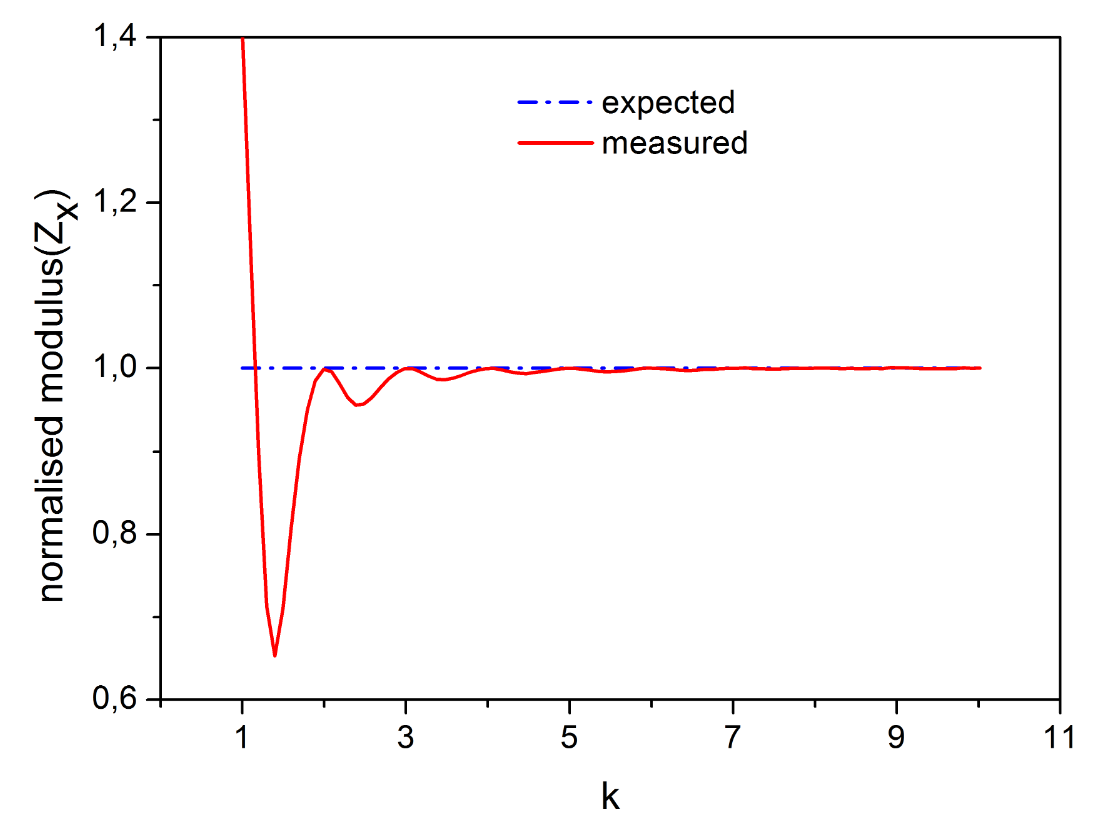
\includegraphics[width=0.7\textwidth]{AD5933_leak}
    \caption{Leakage in the AD5933 IC caused by the DFT \cite{Chabowski2015}.}
    \label{fig:AD5933_leak}
\end{figure}

Lastly, the phase measurement is affected by a systematic error which can be corrected by an adequate calibration of the phase values\cite{Chabowski2015}, as explained in the datasheet of the AD5933 IC \cite{AD5933-documentation}.\par

Notwithstanding these flaws, the AD5933 still distinguishes itself among the scientific community because of its simplicity and convenient packaging. Similar performances are observed between the designs made with dedicated discrete ICs and those obtained with the impedance analyzer IC AD5933. Errors less than $3\%$ are to be expected for measurements of impedance modulus and phase ranging from $10 \Omega$ to over $1 M\Omega$, and for frequencies spanning a couple of hertz to 100 kHz \cite{Al-Ali2017,Sylvain2018,Chabowski2015}. This upper limit for the frequency is fixed by the antialiasing filter attached to the ADC of the IC AD5933. In designs using discrete IC, the upper frequency is similar, and depends on the gain-bandwidth product of the op-amps utilized in its realization. 
